\documentclass[a4paper,11pt]{article}

\usepackage[utf8]{inputenc} \usepackage[T1]{fontenc}
\usepackage{fancyhdr} \usepackage{graphicx,subfig} \usepackage{lastpage}
\usepackage{amssymb,amsmath} \usepackage{siunitx} \usepackage[nodayofweek]{datetime}
\usepackage[top=3.5cm,bottom=2.5cm,left=3cm,right=3cm,headheight=40pt]{geometry}
\usepackage{parskip} \usepackage{float} \usepackage{enumitem} \pagestyle{fancy}
\usepackage[colorlinks=true,allcolors=blue]{hyperref} \hypersetup{
	pdfauthor={Michaël Defferrard},
	pdftitle={Project stage 2: Rendering},
	pdfsubject={Introduction to Computer Graphics}
}

\lhead{Introduction to Computer Graphics\\Project stage 2: Rendering\\Group 19}
\chead{\hspace{2.5cm}EPFL\\\hspace{2.5cm}\shortdate\today\\\hspace{2.5cm}\thepage/\pageref{LastPage}}
\rhead{Michaël \textsc{Defferrard}\\Pierre \textsc{Fechting}\\Vu Hiep \textsc{Doan}}
\cfoot{}

\begin{document}


\section{Overview}

This report presents our advancement on the second part of the project : rendering using procedural methods. Figure~ shows an example of what our actual code base is able to generate. All the minimal steps to display a procedurally generated terrain were successfully completed. We did also implement some other optional suggested methods, like 


\section{Implementation}

\subsection{Improvement on the last stage}

\subsubsection{Parameter tuning for better terrain generation}
In order to find a better terrain, several combination method has been tested. The first idea was to use an hybrid multi fractal method based on 1 minus the absolute value generated by perlin noise. After tuning parameters, we found a terrain counting few lacs and really sharp mountains as shown Figure \ref{hybridmultifractal_terrain}. Such terrain doesn't contain flat plain, therefor we tested a multi fractal method combining perlin and simplex noise as shown Figure \ref{multifractal_perlin_simplex_terrain}. Oppositely to the hybrid multi-fractal, this method generates flat plains but smooth mountains. 
\begin{figure}[H]
	\centering
	\subfloat[Hybrid multi-fractal based on Perlin noise]{
		\label{hybridmultifractal_terrain}
		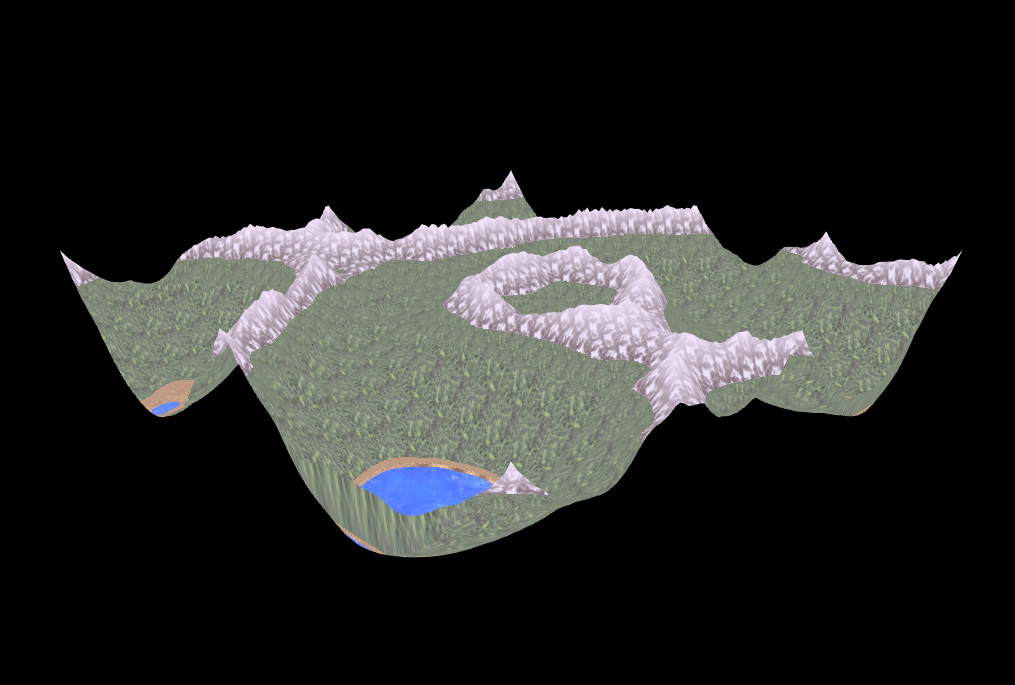
\includegraphics[height=4cm]{{{img_stage2/hybridmultifractal}}}
	} \quad
	\subfloat[Multi-fractal based on perlin and simplex noise]{
		\label{multifractal_perlin_simplex_terrain}
		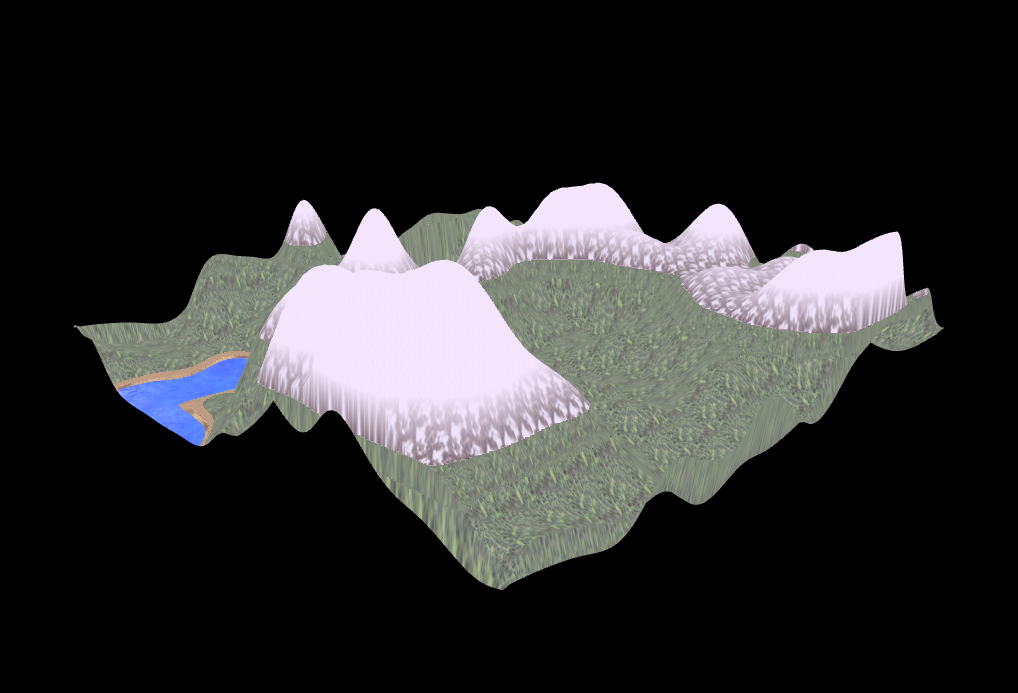
\includegraphics[height=4cm]{{{img_stage2/multifractal_perlin_simplex_noise}}}
	} \quad
	\caption{Terrain generated}
\end{figure}
As we developed several generating method in project part 1, an idea is to combine them.\\
Additive combination: sum the product of a coefficient and the height generated by fractal Brownian motion, multi-fractal (simplex noise based), multi-fractal(perlin noise based), simplex noise and perlin noise. The sum of coefficients must be equal to 1 in order to have a balanced and well scaled terrain. As we have 5 coefficients variating from 0.1 to 1.0, we have 102 possible combinations ( for a sum of coefficient equal to 1). We used an external software called "autoit" to generate the 102 combinations. Using autoit, we wrote a loop setting the coefficients, generating the terrain and saving a snapshot of it. Two example of generated terrain using this method are shown Figures \ref{additive_combination1}, \ref{additive_combination1}.

\begin{figure}[H]
	\centering
	\subfloat[Example 1]{
		\label{additive_combination1}
		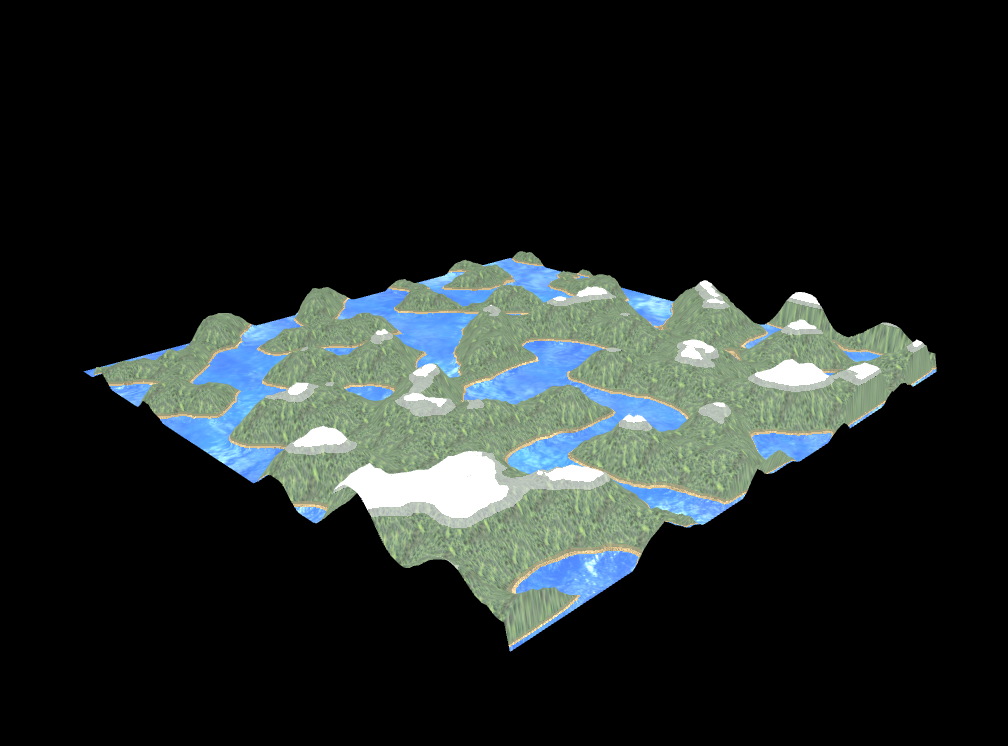
\includegraphics[height=4cm]{{{img_stage2/1_terrain_coefs_0.2_0.4_0.1_0.1_0.2}}}
	} \quad
	\subfloat[Example 2]{
		\label{additive_combination2}
		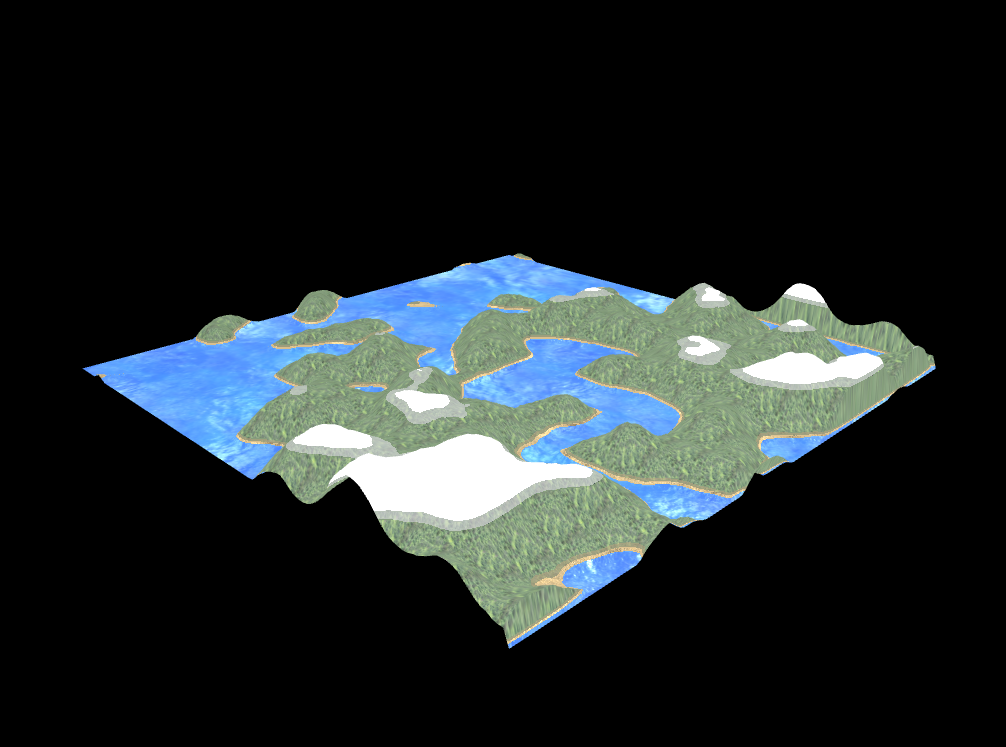
\includegraphics[height=4cm]{{{img_stage2/1_terrain_coefs_0.4_0.2_0.1_0.1_0.2}}}
	} \quad
	\caption{Additive combination}
\end{figure}
Random combination: use different noise and multi-fractal methods according to a randomly generated number. Using randomly a different noise per pixel leads to a highly discontinuous  terrain with abrupt change of height as shown Figure \ref{random_combination}
\begin{figure}[H]
	\centering
	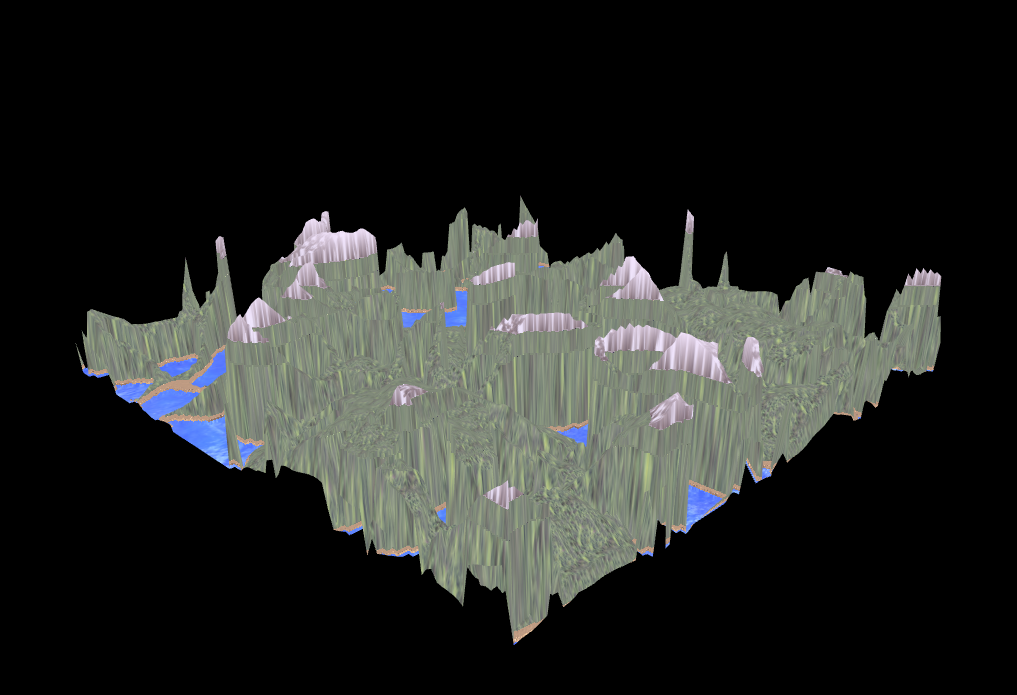
\includegraphics[height=4cm]{{{img_stage2/random_combination}}}
	\caption{Random combination}
	\label{random_combination}
\end{figure}
Spatial combination: use several noise and multi-fractal methods multiplied by a coefficient computed according to the x or y position. This method will smoothly superpose different terrain generation methods creating sharp mountains with lacs and flat plains as shown figures \ref{spatial_combination1} and \ref{spatial_combination2}. 
\begin{figure}[H]
	\centering
	\subfloat[Example 1]{
		\label{spatial_combination1}
		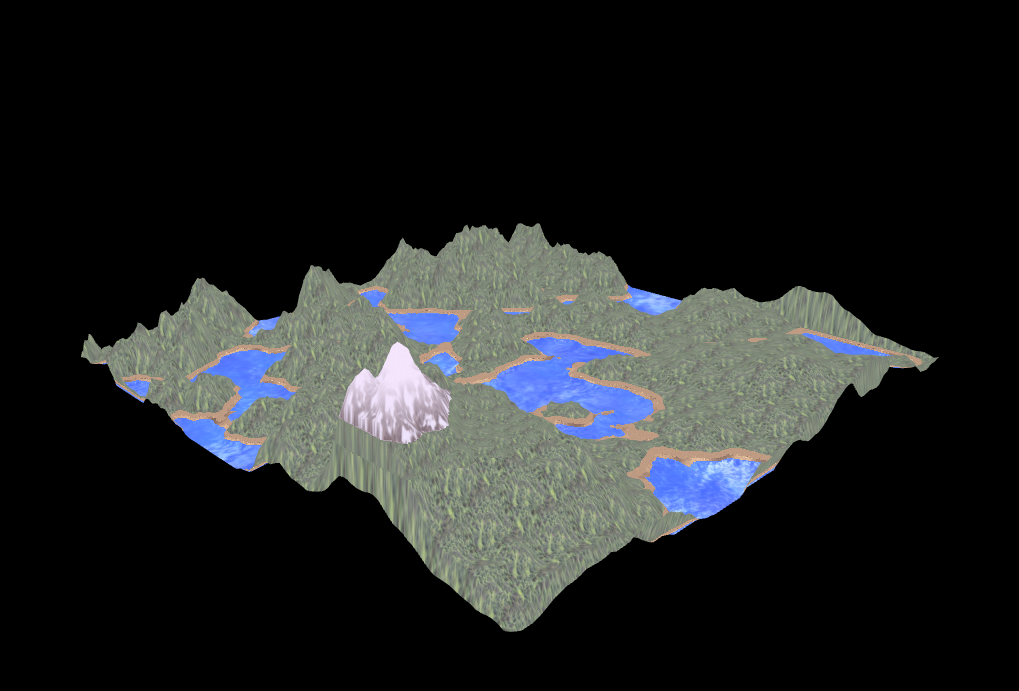
\includegraphics[height=4cm]{{{img_stage2/spatial_combination1}}}
	} \quad
	\subfloat[Example 2]{
		\label{spatial_combination2}
		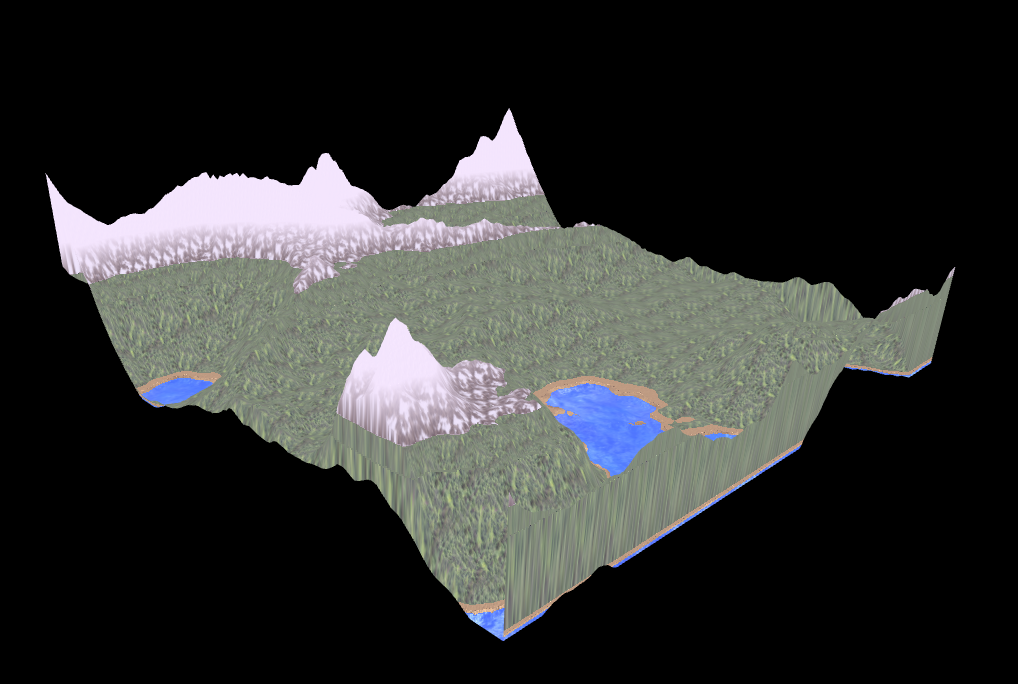
\includegraphics[height=4cm]{{{img_stage2/spatial_combination2}}}
	} \quad
	\caption{Spatial combination}
\end{figure}

\subsubsection{Fixing normal vector calculation}
The normal vector calculation implemented in previous stage is actually not correct but only until we try to blend the texture based on the normal vector that we recognize that the results are not correct. While it costs us a lot of time to re-implement normal vector calculation, the experience that we learned when correcting the normal vector is really invaluable for further understanding OpenGL pipeline.

Firstly, we map the world coordinate to a texel before using \texttt{textureOffset} function to look up the height of surrounding texels in both x and y direction. A finite difference is used to approximate the tangent vector to the surface at that point on the height map then finally, a normal vector will be just the cross product of tangent vectors along x and y directions.

In addition, the above normal vector is just in height map coordinate (ranging from $[0,1] \times [0,1]$ in xy plane) so we need to map it to our world coordinate of the grid ([-1,1] in xy plane). Note that when transform the normal vector, we actually need to multiply it with the inverse of transpose matrix of the transformed one.

To test the normal vector, we output it as the color of each fragment as shown in Figure~\ref{normal_vector}. We can see that the result is quite reasonable, for example in the ground part as it is flat region, the normal vector should be (0,0,1) and as a result, its color is blue.


\begin{figure}[ht]
	\centering
	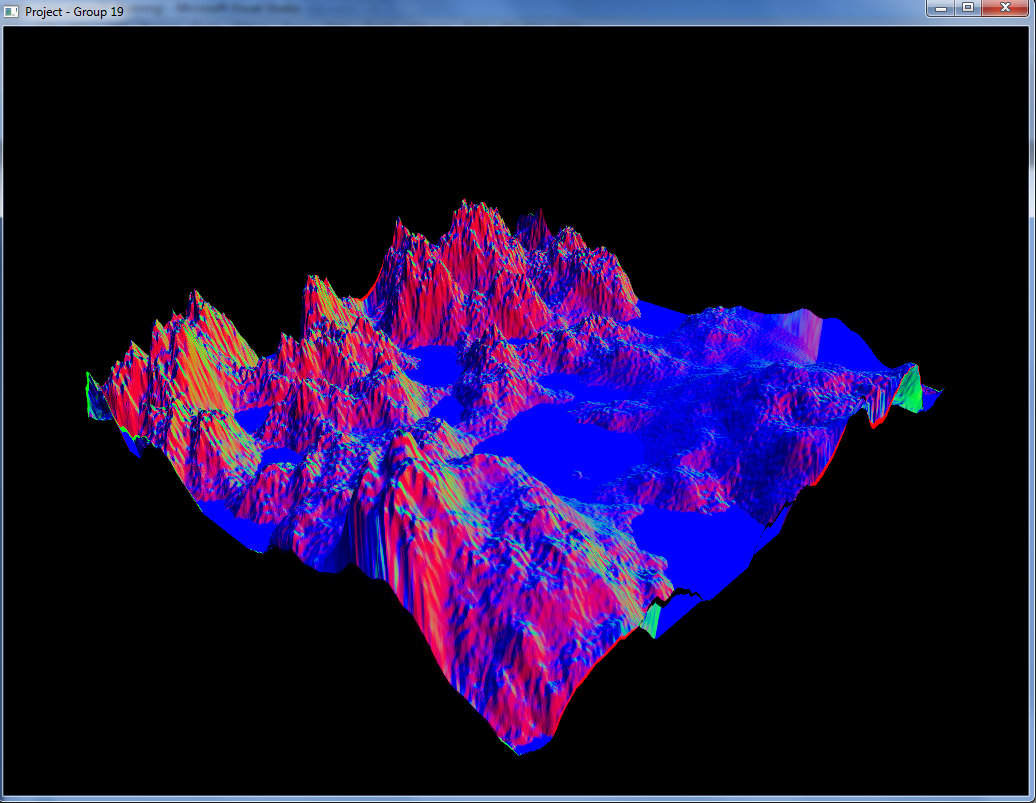
\includegraphics[height=4cm]{{{img_stage2/normal_vector}}}
	\caption{The terrain is colored by its own normal vector.}
	\label{normal_vector}
\end{figure}
\subsection{Basic}
\subsubsection{Texturing}
In this part, our idea is that we can use whatever texture that we want, whatever method or way of blending that we want as long as the terrain looks realistic. Also, the way we implement texture blending is trial and errors, we try many different ways of blending and continue in the direction that generates better results.


\begin{figure}[ht]
	\centering
	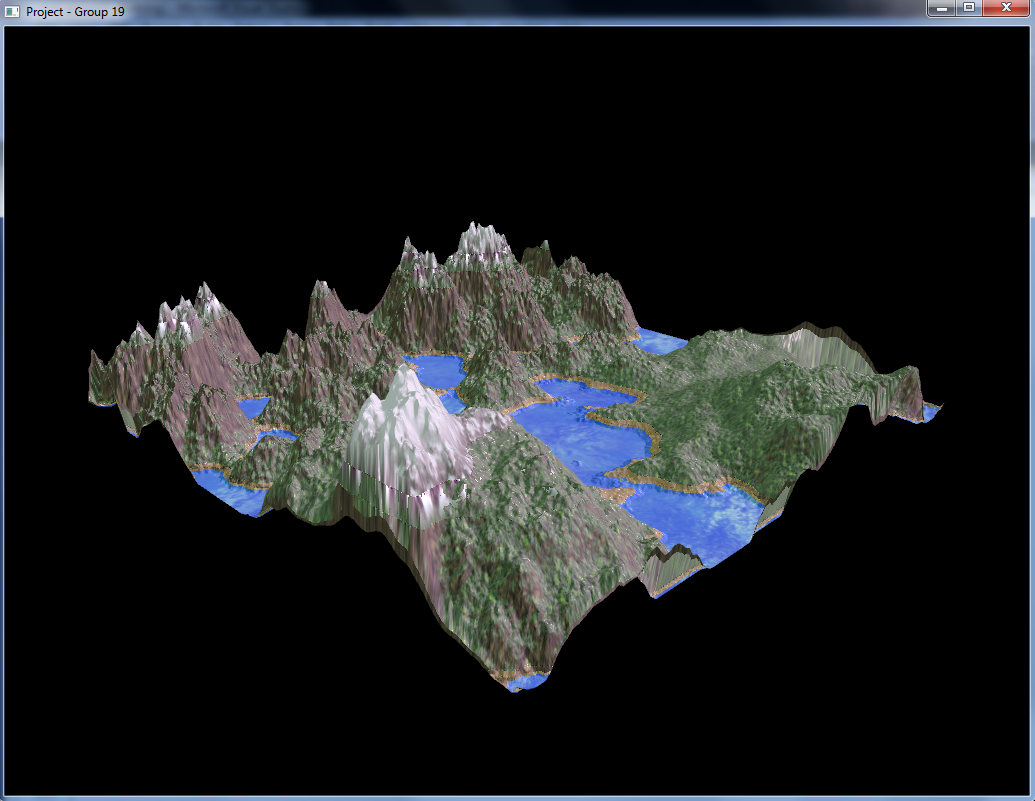
\includegraphics[height=4cm]{{{img_stage2/texture_blending_with_specular}}}
	\caption{The terrain with blended texture.}
	\label{texture_blending}
\end{figure}

\subsubsection{Modeling the sky}

\subsubsection{Self shadowing}


\subsection{Advanced}

\subsubsection{Approximating water reflections/refractions}

\subsubsection{Water depth effect (participating media)}

\subsubsection{Water dynamics}
In order to animate the water texture, we measure time during program execution and send this value through a uniform variable to the fragment shader. This time value will be used to compute an offset applied to the position of the pixel to read in texture.
\subsubsection{Time of the day}


\section{Results}


\end{document}
